\begin{surferPage}[Con Dublu]{Un con dublu}
    A\c{s}a cum s-a explicat in introducerea acestei galerii, o suprafa\c{t}\u{a}
    se nume\c{s}te \emph{nesingular\u{a}} sau neted\u{a} dac\u{a} nu are v\^{a}rfuri
    (astfel de puncte sunt numite singularit\u{a}\c{t}i).
    De exemplu, o sfer\u{a} sau un tor (cele dou\u{a} imagini din st\^{a}nga jos):
        \begin{center}
      \begin{tabular}{@{}c@{}c@{}c@{}c@{}}
        \begin{tabular}{@{}c}
          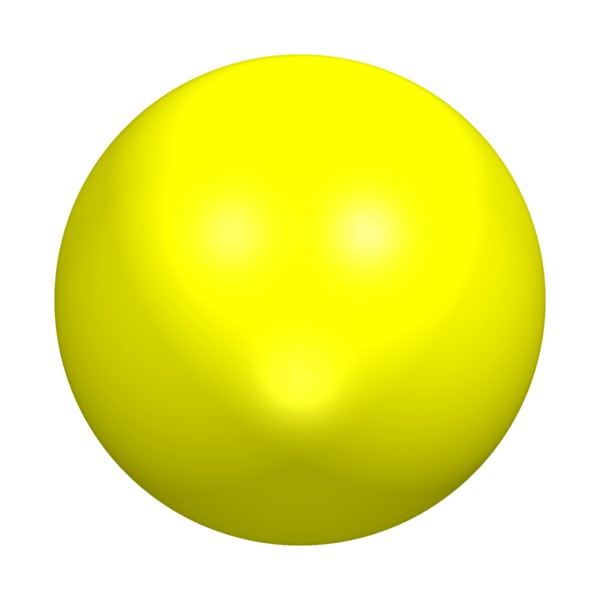
\includegraphics[width=1.4cm]{kugel}
        \end{tabular}
        &
        \begin{tabular}{@{}c}
          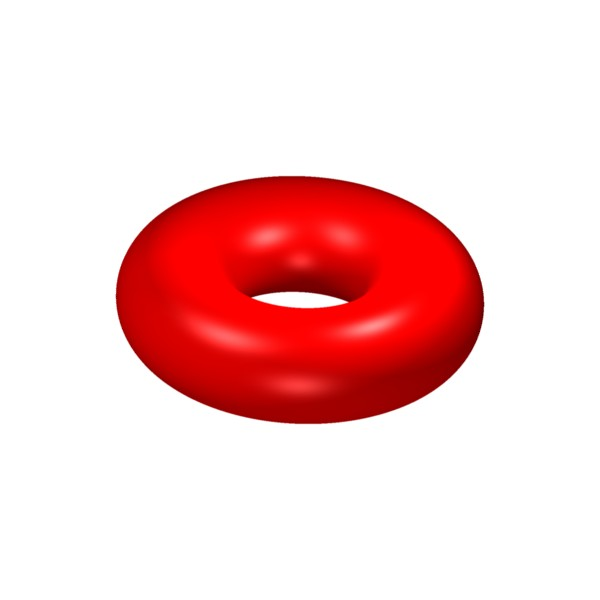
\includegraphics[width=1.4cm]{torus}
        \end{tabular}
        &
        \begin{tabular}{c@{}}
          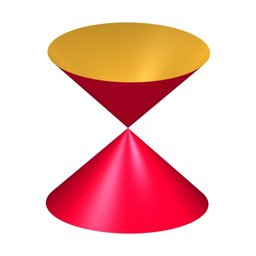
\includegraphics[width=1.4cm]{kegel}
        \end{tabular}
      \end{tabular}
    \end{center}
    Conul dublu (imaginea din dreapta) este cea mai simpl\u{a} singularitate. Este singura singularitate
    care poate fi descris\u{a} printr-o ecuatie de grad $2$:
    \[x^2+y^2-z^2=0.\]
    Atunci c\^{a}nd perturb\u{a}m ecua\c{t}ia prin \^{i}nlocuirea lui $0$ cu o valoare mic\u{a}
    $a \neq 0$, conul dublu se transform\u{a} \^{i}n unul dintre cele doua tipuri de hiperboloide,
    in func\c{t}ie de semnul lui $a$:
    \begin{center}
      \begin{tabular}{@{}c@{\ }c@{\ }c@{\ }c@{\ }c@{}}
        \begin{tabular}{@{}c@{}}
          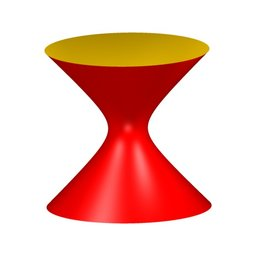
\includegraphics[width=1.2cm]{A1pm_2}
        \end{tabular}
        &
        $\leftarrow$
        &
        \begin{tabular}{@{}c@{}}
          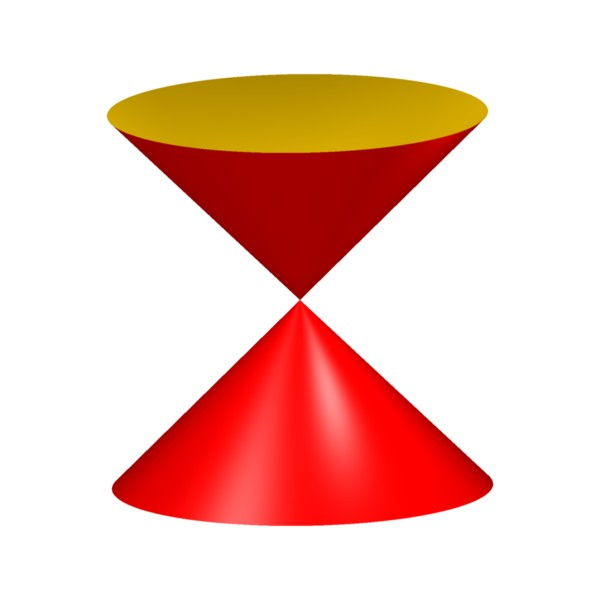
\includegraphics[width=1.2cm]{A1pm_1} 
        \end{tabular}
        &
        $\rightarrow$
        &
        \begin{tabular}{@{}c@{}}
          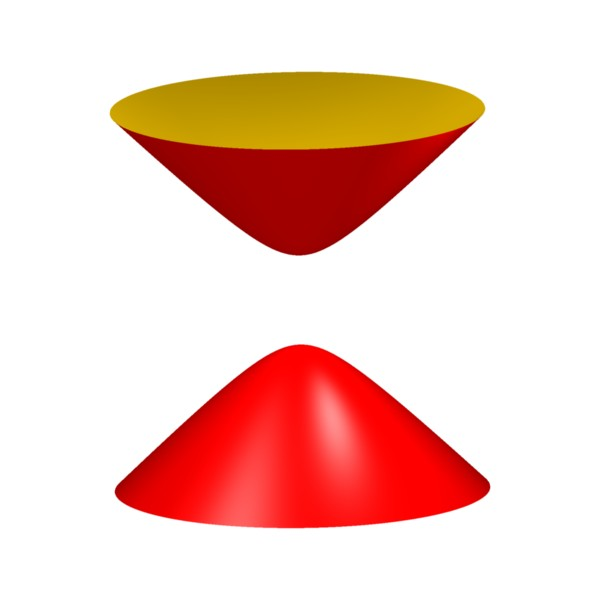
\includegraphics[width=1.2cm]{A1pm_0}
        \end{tabular}
      \end{tabular}
    \end{center}
    O suprafa\c{t}\u{a} de grad $2$ nu poate avea mai mult de o singularitate, adic\u{a} $\mu(2)=1$.
\end{surferPage}
